\documentclass[conference]{IEEEtran}

\usepackage{cite}
\usepackage{amsmath,amssymb,amsfonts}
\usepackage{graphicx}
\usepackage{booktabs}
\usepackage{multirow}
\usepackage{array}
\usepackage{url}
\usepackage{xcolor}
\usepackage{balance}

\graphicspath{{figures/}}

\begin{document}

\title{Leakage-Safe Daily Smart-Meter Forecasting on Small Samples:\\
Benchmarking Tree Ensembles, Deep Models, and Residual Hybrid Refinements}

\author{%
\IEEEauthorblockN{Rohith Ganesh Kanchi}
\IEEEauthorblockA{%
\textit{School of Computing, Department of Computer Science \& Engineering}\\
\textit{VIT Chennai}\\
Chennai, India\\
Reg.\ No.: 23BCE5049\\
Phone: +91 7305636052\\
rohithganesh.kanchi2023@vitstudent.ac.in\\
\url{https://github.com/rZk1809/london-smart-meter-forecasting}}
}

\maketitle

\begin{abstract}
This paper presents a detailed and honest study of daily smart-meter energy forecasting in a small-data setting. The data come from the Low Carbon London smart-meter program. The raw source contains 4,999,863 half-hourly records from 138 households. These readings are aggregated into a single daily total series with 829 rows. After building leakage-safe lag, rolling, calendar, difference, and percentage-change features, 739 usable rows remain. The final modeling split is chronological: 517 rows for training, 110 for validation, and 112 for testing.

The central goal of the project is simple: identify which model class works best for this dataset when the evaluation is fair. To answer that question, the study compares simple baselines, boosted-tree models, Prophet, recurrent neural networks, and several CatBoost-based residual hybrid models. The main result is clear. CatBoost is the strongest overall model on the held-out test set with RMSE 5151.33\,kWh and MAE 1907.47\,kWh. LightGBM and XGBoost are competitive but weaker. GRU and BiLSTM do not beat the tree models. The hybrid residual models are useful as research extensions, but they still do not beat CatBoost on the main metric. Dynamic retrieval residuals nearly tie the backbone, HARP-v2 slightly improves MAE but not RMSE, and CARE improves some secondary behaviors while still lowering overall robustness on RMSE.

The paper explains the full pipeline in simple language: how the dataset was checked, how leakage was prevented, why each model was chosen, what succeeded, what failed, and what the remaining errors mean. The final conclusion is that this dataset behaves more like a small tabular forecasting problem than a large deep-sequence benchmark. Because of that, careful feature engineering and strict chronological evaluation matter more than model complexity. The hardest remaining errors are concentrated in a few rare shock-like days, which suggests that future work should focus on anomaly-aware correction rather than larger neural architectures.
\end{abstract}

\begin{IEEEkeywords}
smart-meter forecasting, load forecasting, CatBoost, tabular time series, small-data forecasting, leakage-safe evaluation, hybrid residual models
\end{IEEEkeywords}

\noindent\textbf{Public repository:} \url{https://github.com/rZk1809/london-smart-meter-forecasting}

\noindent\textbf{Official dataset page:} \url{https://data.london.gov.uk/dataset/smartmeter-energy-consumption-data-in-london-households-vqm0d/}

\noindent\textbf{Low Carbon London project page:} \url{https://innovation.ukpowernetworks.co.uk/projects/low-carbon-london/}

\noindent\textbf{Official dataset source:} \url{https://data.london.gov.uk/dataset/smartmeter-energy-use-data-in-london-households}

\section{Introduction}
Energy forecasting is important because power systems must always balance demand and supply. If demand is predicted too low, the grid may not be prepared. If demand is predicted too high, resources may be wasted. Smart meters make this problem easier to study because they record electricity use at fine time intervals. However, having smart-meter data does not automatically make forecasting easy. Real projects often do not have millions of clean daily training samples. They may only have a few hundred useful observations after data preparation, feature engineering, and leakage-safe splitting.

That small-data reality is the main reason for this study. Many forecasting papers focus on large deep learning models, especially attention-based or transformer-based architectures. Those models are powerful when they have enough data and when the useful patterns are hidden in raw sequences. In this project, the situation is different. The target is a single daily aggregate energy series. The feature engineering pipeline already exposes strong patterns such as recent lags, rolling means, rolling standard deviations, weekday effects, month effects, and short-term changes. Because of that, the problem becomes closer to a structured supervised learning task than a raw representation learning task.

The goal of this paper is therefore not to promote model complexity. The goal is to answer a careful and fair question: \emph{for this exact dataset, under a proper chronological and leakage-safe protocol, which model really works best?} The answer matters for practice. If a simpler model is stronger, then it is a better operational choice. If a more complex model does not improve the main metric, that negative result is still useful because it prevents future work from repeating the same mistake.

The study is guided by three research questions.
\begin{enumerate}
\item Which model family performs best on the canonical daily aggregate smart-meter dataset when the split is strictly chronological?
\item Do residual hybrid refinements improve over a strong CatBoost backbone?
\item What do the remaining errors tell us about the real difficulty of the dataset?
\end{enumerate}

The paper makes four main contributions.
\begin{enumerate}
\item It presents a fully leakage-safe benchmark across statistical baselines, machine learning models, time-series models, and deep learning models.
\item It evaluates three CatBoost-centered residual extensions: DynamicRetrievalResidual, HARP-v2, and CARE.
\item It reports the hybrid results honestly, even though they do not beat CatBoost on the main held-out metric.
\item It explains the final result in plain terms by linking model behavior back to dataset size, feature design, split logic, and shock-day errors.
\end{enumerate}

\section{Problem Statement and Study Logic}
This project studies \emph{one-step-ahead daily aggregate energy forecasting}. For each day $t$, the task is to predict the total energy consumption for that day using only information that would have been available before the day starts. The forecast target is not household-level usage and not half-hourly usage. It is a single aggregate daily value after combining all households.

This choice is important because it defines the type of problem being solved. The dataset is not a large multivariate sensor stream. It is a single daily series with strong periodic behavior and strong calendar structure. That means the forecasting model must do three things well:
\begin{enumerate}
\item use recent history effectively,
\item capture calendar effects such as weekday and season patterns,
\item remain stable when the number of training examples is small.
\end{enumerate}

The project also follows a strict fairness rule. Every model must face the same train, validation, and test windows. No model is allowed to use future values when building features. No model is allowed to tune itself on the test set. The purpose of this rule is simple: a stronger score only matters if it comes from a fair comparison.

There is also a second study logic behind the paper. The project first asks which standard model wins the benchmark. Then it asks whether a more specialized hybrid idea can improve that winner. This leads to a two-step research structure:
\begin{enumerate}
\item build the clean benchmark and identify the strongest base model,
\item add hybrid residual refinements on top of that base model and test whether they help.
\end{enumerate}

That is why CatBoost appears twice in the story: first as a benchmark model, and later as the backbone for the hybrid extensions.

\section{Related Work}
Load forecasting is a long-running problem in energy analytics. Earlier work often used statistical or machine learning models with hand-designed features. More recent work added recurrent networks and attention-based models. This paper does not attempt a full survey. Instead, it uses a focused set of references that directly support the choices made in the project.

The first group of related work covers recurrent models. LSTM networks were introduced to learn long and short temporal dependencies through gated memory cells~\cite{hochreiter1997lstm}. GRU models simplified this idea while keeping the core notion of gated sequence learning~\cite{cho2014gru}. These models have been used in many forecasting tasks, including household energy demand forecasting~\cite{shi2018deep}. Bidirectional recurrent models can sometimes give better sequence representations when the whole sequence is available offline~\cite{schuster1997bilstm}. For that reason, GRU and BiLSTM were included in this benchmark.

The second group of related work covers gradient-boosted trees. XGBoost~\cite{chen2016xgboost}, LightGBM~\cite{ke2017lightgbm}, and CatBoost~\cite{dorogush2018catboost} are standard strong baselines for structured regression problems. They are especially useful when the feature matrix already captures the important signal. This is relevant here because the project builds many informative lag, rolling, and calendar predictors before model fitting. Grinsztajn \emph{et al.}~\cite{grinsztajn2022tree} argue that tree-based models still outperform deep learning on many tabular datasets, especially when the data are not huge and when the input features are already highly informative. That claim is directly relevant to the results in this paper.

The third group covers recent attention and transformer-style forecasting. The original attention-based transformer architecture~\cite{vaswani2017attention} strongly influenced later time-series work, including PatchTST~\cite{nie2023patchtst}. At the same time, Zeng \emph{et al.}~\cite{zeng2023transformers} question whether transformer-style models are always the right choice for time-series forecasting. Their argument is useful for this paper because the present dataset is much smaller than the large benchmark settings where such architectures are often tested.

Finally, a proper forecasting study needs a proper evaluation design. Bergmeir \emph{et al.}~\cite{bergmeir2018validity} discuss the validity of resampling methods in autoregressive settings and highlight the importance of respecting time order. This point is central here. In time-series forecasting, a model can appear better than it really is if rolling features, lag features, or validation logic accidentally use future information. This paper treats leakage prevention as a core methodological requirement, not an implementation detail.

\section{Dataset, Data Validation, and Problem Formulation}
\subsection{Raw data source}
The data used in this project come from the Low Carbon London smart-meter program~\cite{lcl2014}. The inherited raw audit stored in the repository reports 4,999,863 half-hourly readings collected from 138 households between 23 November 2011 and 28 February 2014. This raw file is not used directly for modeling in the final benchmark. Instead, it serves as the source from which the canonical daily aggregate dataset was built.

\begin{table}[t]
\caption{Dataset audit from raw source to final feature frame.}
\label{tab:data_audit}
\centering
\begin{tabular}{p{4.2cm}r}
\toprule
\textbf{Audit item} & \textbf{Value} \\
\midrule
Raw half-hourly rows & 4,999,863 \\
Unique households & 138 \\
Raw missing values & 0 \\
Raw outliers (IQR rule) & 8.99\% \\
Daily aggregate rows & 829 \\
Processed daily missing values & 0 \\
Processed duplicate dates & 0 \\
Feature-ready rows & 739 \\
Feature-frame columns & 53 \\
Leakage-safe predictors & 51 \\
\bottomrule
\end{tabular}
\end{table}

\subsection{Canonical daily dataset}
The final modeling file is \texttt{data/processed/daily\_agg.parquet}. It contains only two columns: \texttt{ds} for date and \texttt{y} for daily total energy. The file has 829 rows, one for each day from 23 November 2011 to 28 February 2014. A direct local check shows that this file has no missing targets and no duplicate dates. The daily mean is 42,895.91\,kWh and the daily standard deviation is 20,152.11\,kWh. The minimum value is 90.39\,kWh and the maximum is 82,650.49\,kWh.

These checks matter because they answer a basic validation question: \emph{is the dataset trustworthy enough to model?} In this project, the answer is yes for three simple reasons:
\begin{enumerate}
\item the processed daily file is complete and has no missing target values,
\item every day appears only once,
\item the date range is continuous and long enough to show weekly, monthly, and seasonal behavior.
\end{enumerate}

\subsection{Why the dataset is valid for this project}
The dataset is valid for a daily forecasting project because it matches the final prediction target. The project is not trying to forecast each household separately. It is trying to forecast the \emph{total daily demand} of the full smart-meter group. For that goal, daily aggregation is a reasonable and useful transformation. It removes some noise from half-hourly readings and shifts the problem toward operational planning at the daily scale.

The dataset is also valid because it contains clear structure. Weekend days are higher on average than weekdays: 44,329.06\,kWh versus 42,325.55\,kWh. The autocorrelation is very high at short and weekly lags: approximately 0.991 at lag 1, 0.983 at lag 7, and 0.950 at lag 28. These values show that the series contains strong memory and repeatable patterns, which is exactly what a forecasting model needs.

At the same time, the dataset is not easy. The series also shows drift across time and a few extreme events. That makes it a good test case for model comparison because it contains both regular patterns and difficult rare cases.

\subsection{Formal problem definition}
Let $y_t$ denote the aggregate daily energy value on day $t$. Let $c_t$ denote the calendar variables for day $t$, such as weekday, month, and season indicators. Let the leakage-safe feature map be written as
\begin{equation}
x_t = \phi(y_{<t}, c_t).
\end{equation}
The forecasting task is then to learn a function
\begin{equation}
\hat{y}_t = f(x_t),
\end{equation}
where $\hat{y}_t$ is the predicted daily energy for day $t$.

For the hybrid models, the forecast is written as a base prediction plus a residual correction:
\begin{equation}
\hat{y}_t = \hat{y}^{cb}_t + \hat{r}_t,
\end{equation}
where $\hat{y}^{cb}_t$ is the CatBoost forecast and $\hat{r}_t$ is the learned residual adjustment.

\subsection{Chronological split}
The final split is strict and chronological. No row from the future is allowed to influence training or validation.

\begin{table}[t]
\caption{Chronological split used in all final comparisons.}
\label{tab:split_summary}
\centering
\begin{tabular}{lrr}
\toprule
\textbf{Split} & \textbf{Rows} & \textbf{Date range} \\
\midrule
Train & 517 & 2012-02-21 to 2013-07-21 \\
Validation & 110 & 2013-07-22 to 2013-11-08 \\
Test & 112 & 2013-11-09 to 2014-02-28 \\
\bottomrule
\end{tabular}
\end{table}

This split is important for two reasons. First, it mirrors real forecasting use, where tomorrow must be predicted using only past data. Second, it prevents hidden leakage from shuffling or random train-test splits.

\section{Methodology}
\subsection{Overall pipeline}
The pipeline used in this project follows a simple sequence:
\begin{enumerate}
\item validate the processed daily dataset,
\item build leakage-safe features,
\item split the data chronologically,
\item train baseline, machine learning, and deep learning models,
\item identify the strongest benchmark model,
\item build hybrid residual refinements on top of that benchmark winner,
\item evaluate all results on the same held-out test set.
\end{enumerate}

This pipeline was chosen because it is easy to explain, easy to reproduce, and suitable for academic review.

\subsection{Feature engineering}
The most important design choice in the project is the feature engineering step. Instead of feeding the raw series directly to every model, the project constructs a supervised feature frame. This frame contains 53 columns: the date, the target, and 51 predictors.

\begin{table}[t]
\caption{Feature groups used in the supervised models.}
\label{tab:feature_groups}
\centering
\begin{tabular}{p{2.0cm}cp{4.3cm}}
\toprule
\textbf{Group} & \textbf{Count} & \textbf{Examples} \\
\midrule
Calendar & 11 & dayofweek, month, quarter, dayofyear, weekofyear, is\_weekend, sine/cosine cycles \\
Lags & 11 & lag\_1, lag\_2, lag\_3, lag\_7, lag\_14, lag\_21, lag\_28, lag\_30, lag\_60, lag\_90 \\
Rolling stats & 25 & mean, std, min, max, median on 3, 7, 14, 21, and 30 day windows \\
Differences & 3 & diff\_1, diff\_7, diff\_30 \\
Pct.\ change & 2 & pct\_change\_1, pct\_change\_7 \\
\midrule
\textbf{Total} & \textbf{51} &  \\
\bottomrule
\end{tabular}
\end{table}

The reason for using these features is simple. Daily demand usually depends on:
\begin{enumerate}
\item what happened very recently,
\item what happened on the same weekday in previous weeks,
\item whether demand is rising or falling,
\item whether the day is a weekday, weekend, or part of a seasonal period.
\end{enumerate}

The chosen features capture exactly these effects in a direct way. This is one of the main reasons the boosted-tree models work well here.

\subsection{Leakage prevention}
The paper makes a strong claim about fairness, so it must explain leakage prevention clearly. Leakage was controlled in three ways.

First, every lag feature uses only earlier target values. Second, every rolling statistic is built from \texttt{shift(1)} history. This means the statistic for day $t$ is computed only from days before $t$. Third, the train, validation, and test splits are applied in time order, and no tuning is done on the test set.

This design is important because time-series leakage can happen silently. For example, if a rolling mean includes day $t$, then the model can indirectly see the target it is trying to predict. That would make the results look better than they really are. The repository code explicitly avoids this problem.

\subsection{Why these models were selected}
The model list was chosen to answer a practical question, not just a research-fashion question. Each model class plays a clear role.

\begin{table}[t]
\caption{Why each model family was included.}
\label{tab:model_rationale}
\centering
\begin{tabular}{p{1.6cm}p{5.4cm}}
\toprule
\textbf{Family} & \textbf{Purpose in the study} \\
\midrule
Baselines & Give a simple lower bound and show how hard the task really is. \\
Boosted trees & Test strong nonlinear tabular models on the engineered feature frame. \\
Prophet & Provide a well-known forecasting baseline with trend and seasonality structure. \\
GRU/BiLSTM & Test whether sequence models can discover extra structure beyond the engineered features. \\
Hybrids & Test whether CatBoost errors can be corrected by targeted residual modeling. \\
\bottomrule
\end{tabular}
\end{table}

This table also answers another common question: \emph{is the person working on the project choosing the right models for the dataset?} The answer is yes, because the selected models cover simple benchmarks, strong tabular learners, classical time-series structure, deep sequence models, and advanced hybrid extensions. That gives a balanced comparison.

\subsection{Baseline models}
Three simple baselines were used.

\textbf{Naive} uses the previous day as the forecast:
\begin{equation}
\hat{y}_t = y_{t-1}.
\end{equation}

\textbf{Seasonal Naive} uses the same weekday from the previous week:
\begin{equation}
\hat{y}_t = y_{t-7}.
\end{equation}

\textbf{Moving Average 7} uses the average of the previous seven days:
\begin{equation}
\hat{y}_t = \frac{1}{7}\sum_{i=1}^{7} y_{t-i}.
\end{equation}

These models are simple, but they are necessary. If a complex model cannot beat them, then the complex model has no practical value.

\subsection{Machine learning models}
The main machine learning models are XGBoost, LightGBM, and CatBoost. All three are gradient-boosted tree methods. In simple words, they build many small trees and combine them into one strong nonlinear predictor. The general boosting idea can be written as
\begin{equation}
\mathcal{L}^{(m)} = \sum_{i=1}^{N}\ell\!\left(y_i,\hat{y}^{(m-1)}_i + f_m(x_i)\right) + \Omega(f_m),
\end{equation}
where $f_m$ is the new tree added at stage $m$.

These models were expected to work well because the feature matrix is already rich and structured. CatBoost was especially promising because it is usually strong on tabular regression and handles ordered data carefully. That expectation was confirmed by the final results.

\subsection{Deep learning models}
Two recurrent deep learning models were evaluated: GRU and BiLSTM.

A GRU updates its hidden state through gated sequence operations. In simple form,
\begin{equation}
h_t = \mathrm{GRU}(x_t, h_{t-1}), \qquad \hat{y}_t = Wh_t + b.
\end{equation}

The BiLSTM uses two recurrent passes, one forward and one backward, and then combines them before the output. In offline sequence tasks this can be useful because it learns richer internal representations.

These models were included because deep recurrent networks are commonly used in energy forecasting. However, the project did not assume they would win. Their role was to test whether the dataset still contains hidden sequential structure that the engineered feature frame might miss.

\subsection{Hybrid residual models}
After CatBoost emerged as the strongest benchmark model, the project explored residual hybrid refinements. The logic is simple. Instead of replacing CatBoost, the hybrid model keeps CatBoost as the base forecast and tries to learn only the remaining error.

\subsubsection{DynamicRetrievalResidual}
This model retrieves historically similar past days and uses them to estimate a residual correction. The core idea is that if the current query day looks like certain days in the past, then the past residual behavior may help correct the CatBoost forecast.

\subsubsection{HARP-v2}
HARP-v2 is a more structured residual retrieval model. It uses a combination of query-key similarity, calendar matching, regime matching, and peak matching:
\begin{equation}
e(t,\tau)=\frac{q_t^\top k_\tau}{\sqrt{d}}+\lambda_{\mathrm{cal}}C(t,\tau)+\lambda_{\mathrm{reg}}R(t,\tau)+\lambda_{\mathrm{peak}}P(t,\tau).
\end{equation}

In simple words, HARP-v2 tries to retrieve past days that are close in three ways:
\begin{enumerate}
\item they happen in a similar calendar context,
\item they come from a similar demand regime,
\item they behave like a similar peak or transition day.
\end{enumerate}

\subsubsection{CARE}
CARE is an accuracy-first residual hybrid. It blends two residual estimates:
\begin{enumerate}
\item an analog residual from similar past days,
\item a linear residual from a compact ridge-style model.
\end{enumerate}
The final prediction is
\begin{equation}
\hat{y}_t = \hat{y}^{cb}_t + g_t\!\left(\alpha r^{\mathrm{analog}}_t + (1-\alpha)r^{\mathrm{linear}}_t\right),
\end{equation}
where $\alpha$ is a blend weight and $g_t$ is a shrinkage gate between 0 and 1.

The purpose of CARE is not to be more complex than HARP-v2. The purpose is the opposite: to see whether a simpler residual correction scheme can improve accuracy more reliably.

\section{Experimental Setup}
\subsection{Training environment}
The benchmark models were run in the repository's canonical pipeline, and the hybrid residual models were rerun in the current environment. The verified hybrid runtime report shows:
\begin{itemize}
\item resolved device: CUDA,
\item GPU: NVIDIA GeForce RTX 3060 Laptop GPU,
\item PyTorch version: 2.7.1+cu118,
\item AMP disabled for stability.
\end{itemize}

This setup matters because it confirms that the hybrid runs were real, reproducible executions and not only paper-level designs.

\subsection{Training policy}
All models use the same target and the same chronological split. Prophet is the only exception in terms of feature input, because it uses only the date and target in its native format. The other models use the same engineered feature frame, which keeps the benchmark fair.

The tree models use a validation-based model selection process. The deep learning models use early stopping. The hybrid models use CatBoost as the backbone and then learn residuals only from leakage-safe train or train-plus-validation logic, depending on the exact stage of the pipeline. Test labels are never used for calibration.

\subsection{Evaluation metrics}
The project reports multiple metrics because no single metric tells the whole story.

\textbf{RMSE} is the main metric:
\begin{equation}
\mathrm{RMSE}=\sqrt{\frac{1}{N}\sum_{t=1}^{N}(y_t-\hat{y}_t)^2}.
\end{equation}
This metric gives more weight to large errors.

\textbf{MAE} is the main robustness metric:
\begin{equation}
\mathrm{MAE}=\frac{1}{N}\sum_{t=1}^{N}|y_t-\hat{y}_t|.
\end{equation}
This metric is easier to explain because it measures the average absolute error directly.

The project also reports MAPE, SMAPE, $R^2$, median absolute error, and direction accuracy. These extra metrics help show whether a model is consistently good or only good under one measure.

\subsection{Hard-case and high-volatility evaluation}
The project adds two focused error slices because overall averages can hide important behavior.

\textbf{High-volatility slice.} A rolling volatility measure is computed using past behavior. This slice isolates periods where the series is more unstable than usual.

\textbf{Hard-case slice.} Hard cases are defined using the 90th percentile of CatBoost validation absolute error. This threshold is 2268.81\,kWh. The resulting definition identifies 18 hard cases in the 112-row test set. This approach is careful because the threshold is defined on validation data, not on the test set.

\section{Results}
\subsection{Main benchmark across standard models}
Table~\ref{tab:main_benchmark} gives the main benchmark. CatBoost is the best overall model. It achieves the lowest RMSE and the lowest MAE among the standard benchmark models. LightGBM and XGBoost are the next strongest models, which supports the idea that this dataset is best handled as a tabular supervised problem.

\begin{table*}[t]
\caption{Main benchmark under the canonical leakage-safe protocol. Lower RMSE and MAE are better.}
\label{tab:main_benchmark}
\centering
\begin{tabular}{lrrrrrrrr}
\toprule
\textbf{Model} & \textbf{RMSE} & \textbf{MAE} & \textbf{MAPE} & \textbf{SMAPE} & \textbf{$R^2$} & \textbf{MedAE} & \textbf{Dir.\ Acc.} & \textbf{Rank} \\
\midrule
CatBoost & \textbf{5151.33} & \textbf{1907.47} & \textbf{24.07} & \textbf{4.135} & \textbf{0.254} & 1274.23 & 57.66 & 1 \\
LightGBM & 5348.21 & 2259.39 & 24.66 & 4.708 & 0.196 & \textbf{1232.66} & 51.35 & 2 \\
XGBoost & 5387.16 & 2139.49 & 25.13 & 4.498 & 0.184 & 1246.16 & 50.45 & 3 \\
GRU & 5610.57 & 2489.04 & 26.13 & 5.098 & 0.115 & 1775.07 & \textbf{64.86} & 4 \\
BiLSTM & 5704.57 & 2965.88 & 25.84 & 5.988 & 0.085 & 2197.45 & 63.06 & 5 \\
Naive & 15531.36 & 15079.55 & 42.78 & 30.397 & -5.781 & 14918.60 & 52.25 & 6 \\
Seasonal Naive & 15575.58 & 15130.89 & 42.87 & 30.515 & -5.819 & 14918.60 & 51.35 & 7 \\
Moving Average 7 & 16292.83 & 15886.29 & 43.83 & 32.241 & -6.462 & 15740.00 & 52.25 & 8 \\
Prophet & 37716.75 & 36769.18 & 64.23 & 96.978 & -38.987 & 37105.14 & 65.77 & 9 \\
\bottomrule
\end{tabular}
\end{table*}

\begin{figure}[t]
\centering
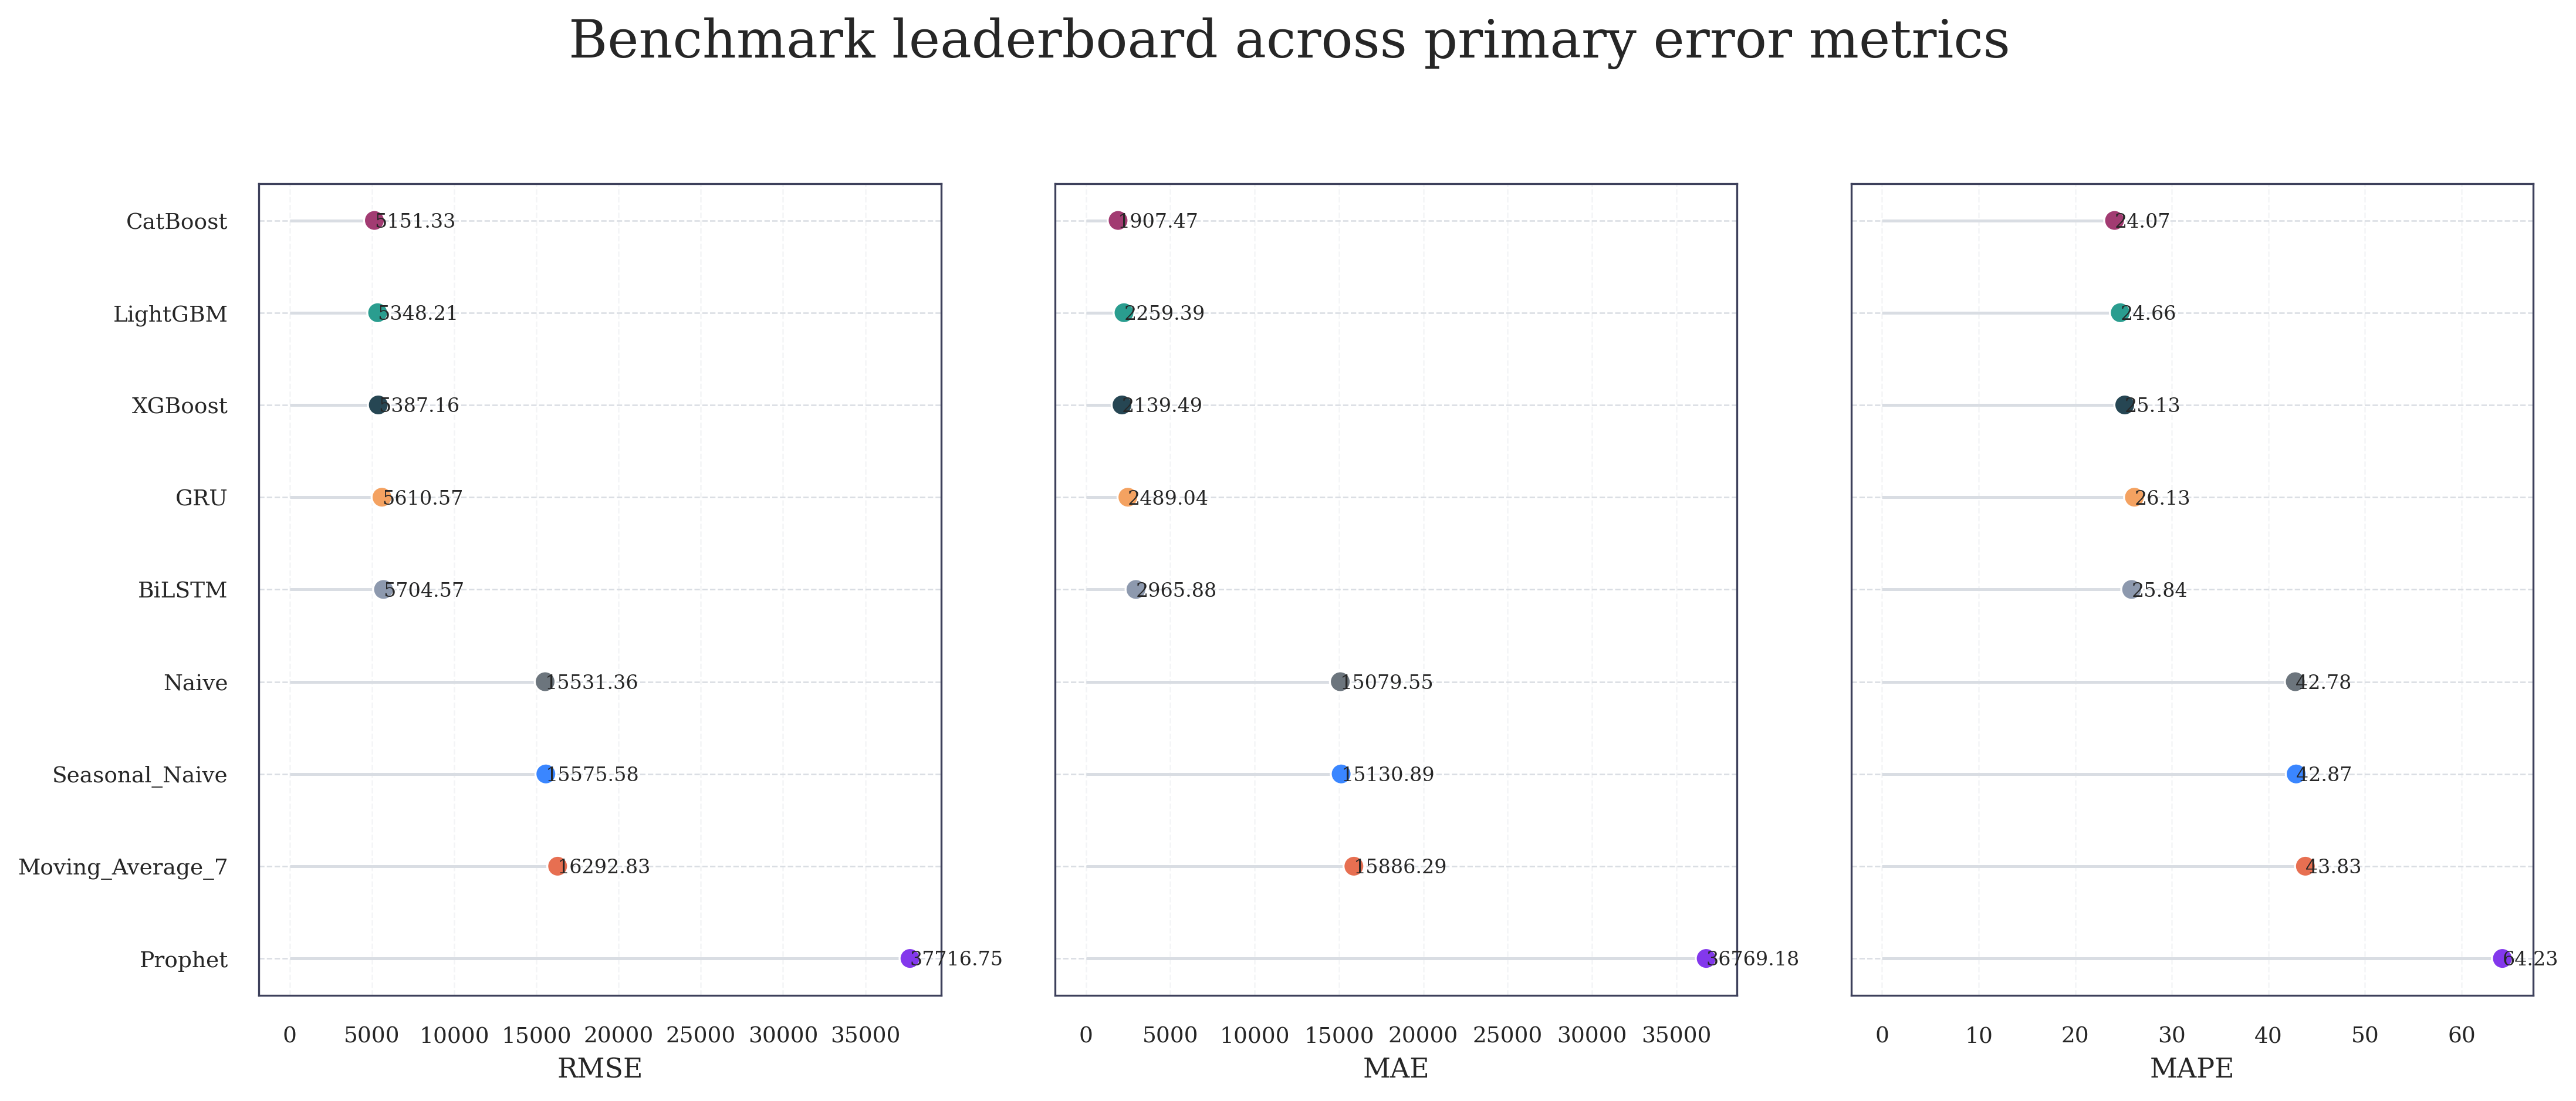
\includegraphics[width=\columnwidth]{benchmark_leaderboard.png}
\caption{Benchmark ranking by RMSE. CatBoost is the strongest model, and the top three methods are all boosted-tree models.}
\label{fig:benchmark_leaderboard}
\end{figure}

\begin{figure}[t]
\centering
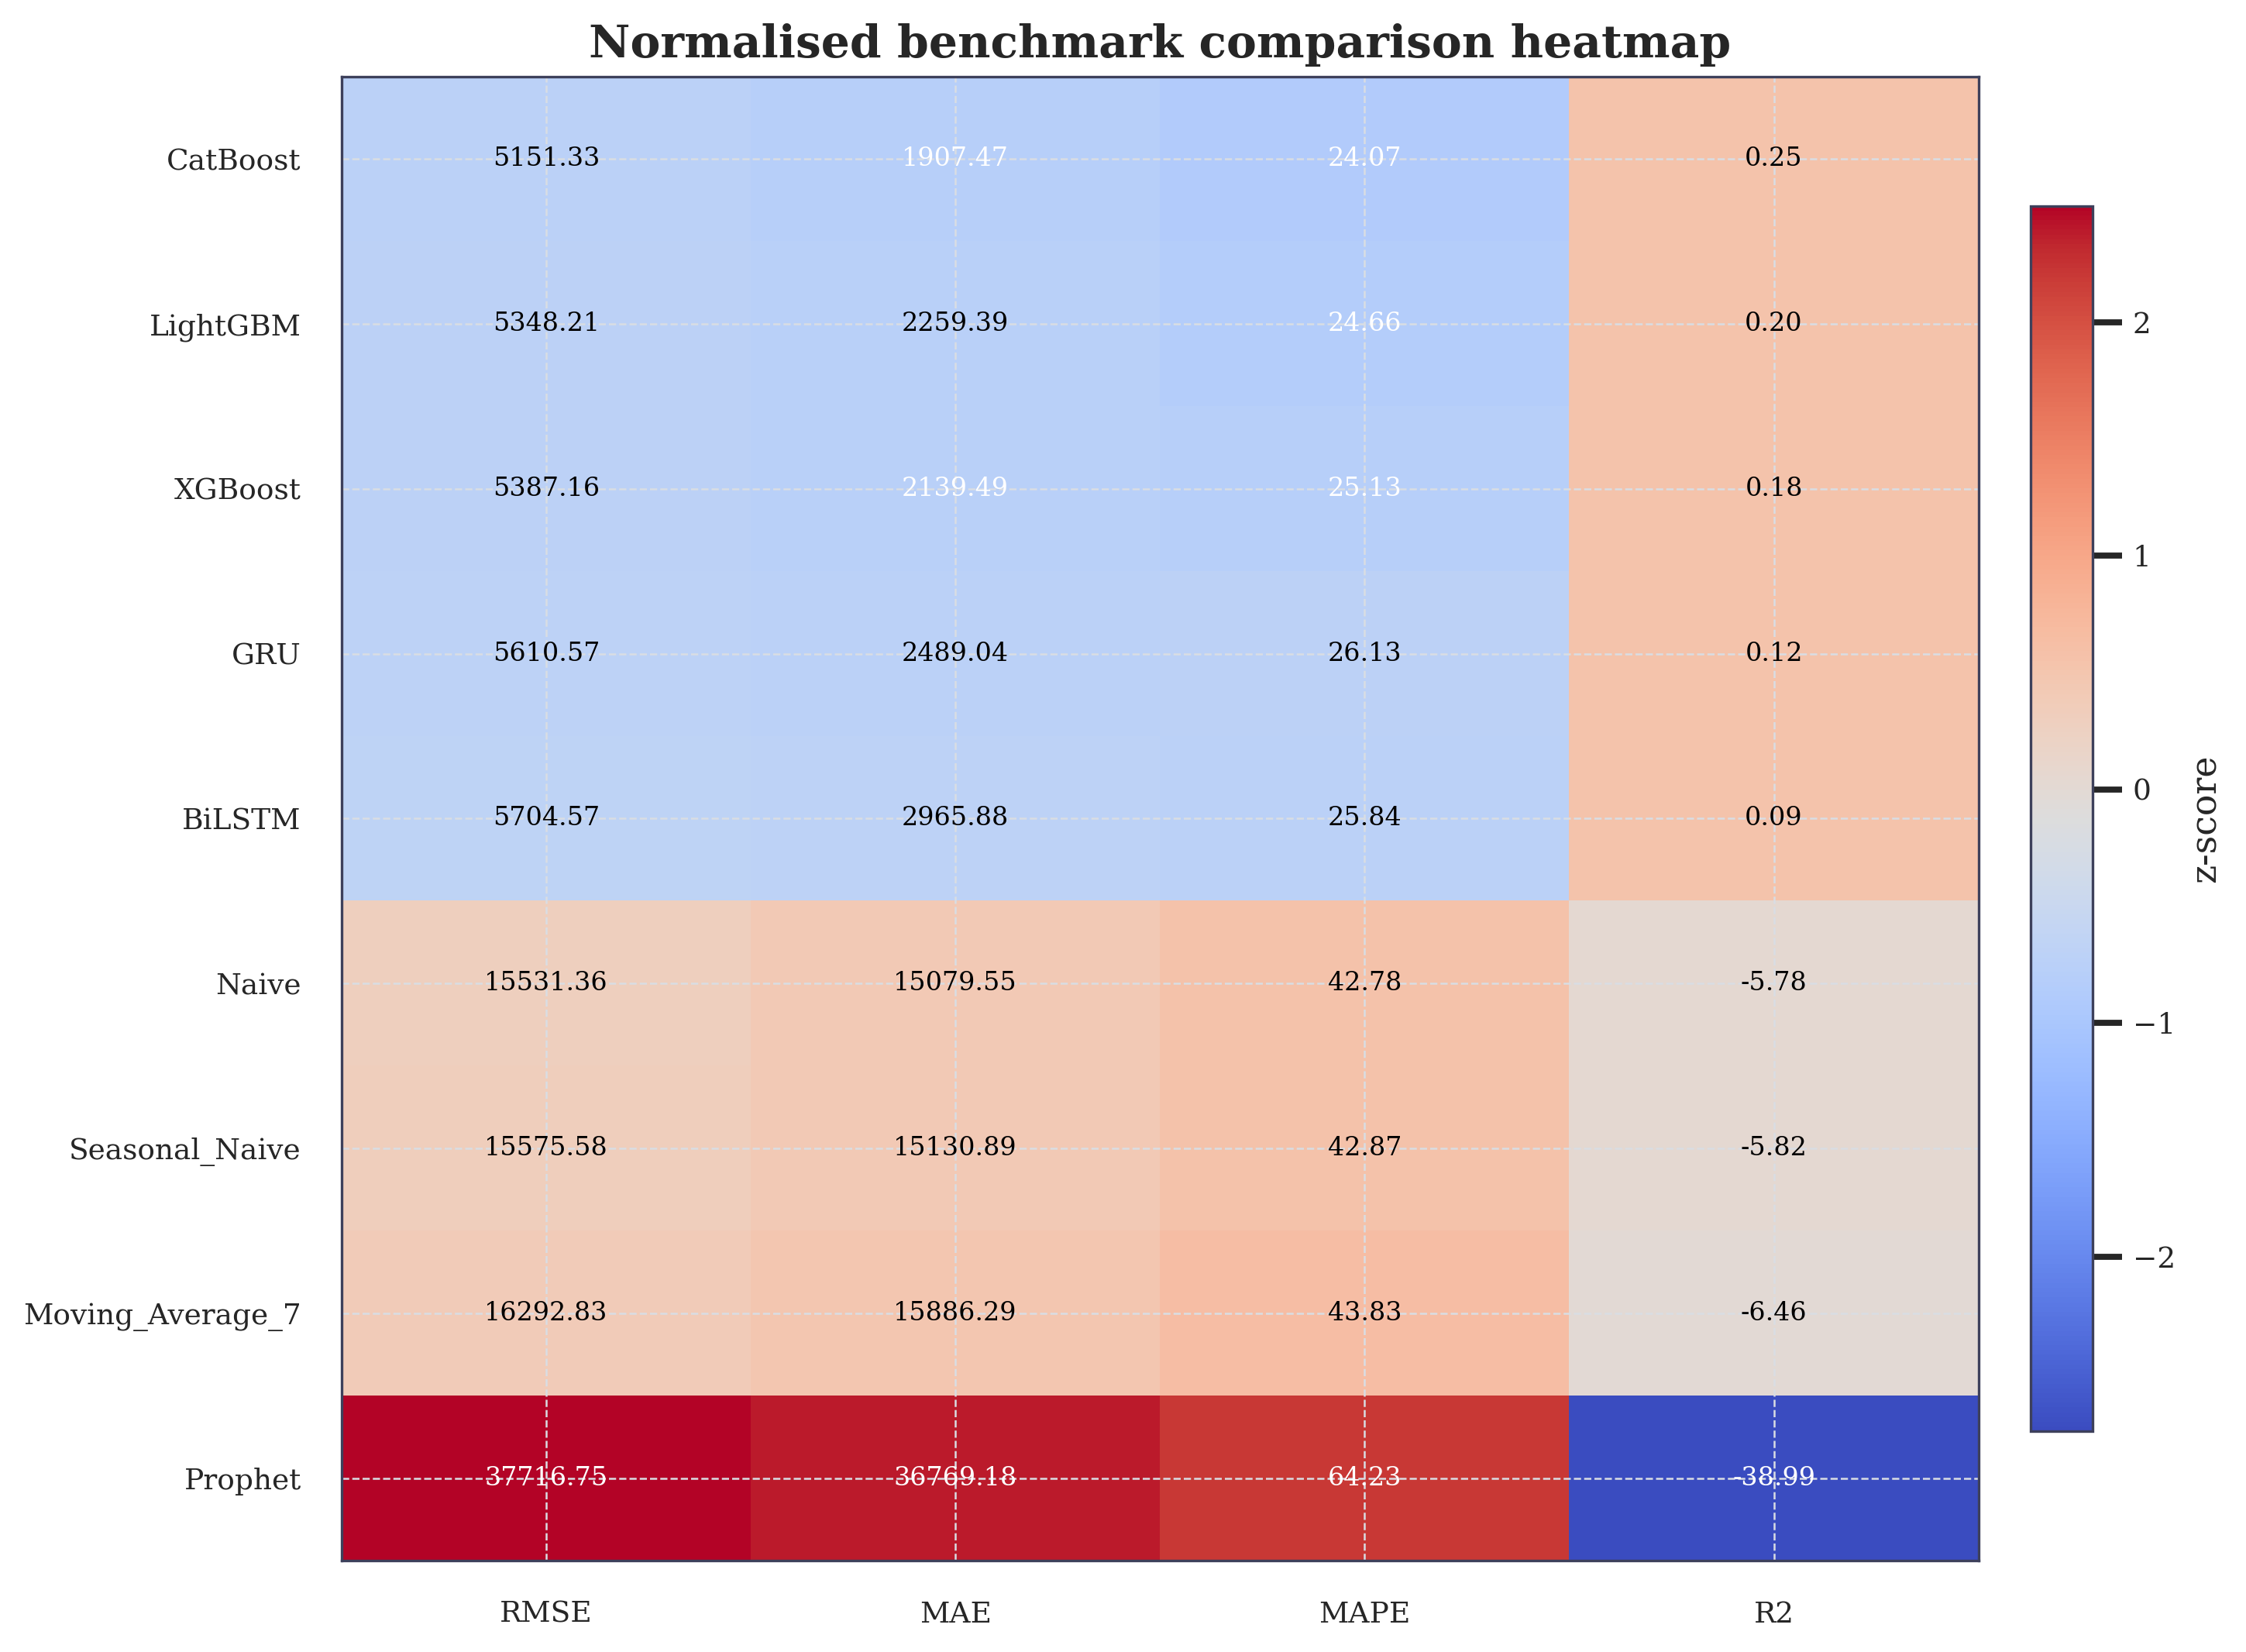
\includegraphics[width=\columnwidth]{benchmark_heatmap.png}
\caption{Benchmark heatmap across metrics. The figure shows that CatBoost is not only the RMSE leader, but also one of the most balanced models across metrics.}
\label{fig:benchmark_heatmap}
\end{figure}

\subsection{What succeeded in the benchmark}
Three findings stand out from the main benchmark.

First, the three boosted-tree models clearly separate themselves from the deep learning models. This is strong evidence that the engineered feature frame is doing important work. Once the signal is expressed as lags, rolling summaries, and calendar terms, the tree models can use it efficiently.

Second, CatBoost is not just slightly better than weak baselines. It is far better than Naive, Seasonal Naive, Moving Average 7, and Prophet. This shows that the task is not trivial and that a proper nonlinear supervised model is needed.

Third, even though GRU and BiLSTM are respectable models, they do not beat CatBoost. This does not mean recurrent models are bad in general. It means they are not the best fit for this exact dataset and this exact feature-and-split design.

\subsection{What did not succeed, and why}
The most obvious underperformer is Prophet. This result is not surprising because the series has strong nonlinear and local variation that is better handled by feature-rich supervised models than by a simple trend-and-seasonality decomposition.

The simple baselines also underperform strongly. This shows that daily smart-meter demand is not captured well enough by only yesterday's value or a simple weekly carry-over rule.

The deep learning models do not fail completely, but they do not justify their extra complexity. GRU and BiLSTM achieve much worse RMSE and MAE than CatBoost. This suggests that the dataset is too small to reward large representation learning capacity.

\subsection{Hybrid residual experiments}
After CatBoost won the main benchmark, the project explored whether its remaining error could be improved through residual correction. This led to DynamicRetrievalResidual, HARP-v2, and CARE.

\begin{table}[t]
\caption{Main hybrid results relative to CatBoost.}
\label{tab:hybrid_main}
\centering
\begin{tabular}{p{3.2cm}rr}
\toprule
\textbf{Model} & \textbf{RMSE} & \textbf{MAE} \\
\midrule
CatBoost & \textbf{5151.33} & 1907.47 \\
DynamicRetrievalResidual & 5151.68 & 1901.90 \\
HARP-v2 Full & 5153.86 & 1891.06 \\
CARE No Conf.\ Abstention & 5182.10 & \textbf{1800.68} \\
CARE Full & 5227.52 & 1861.99 \\
\bottomrule
\end{tabular}
\end{table}

This table tells an important story. The hybrid models are not useless. In fact, they show that residual correction can improve some secondary behavior. For example, HARP-v2 improves MAE slightly compared with CatBoost. CARE without confidence abstention gets the best MAE in the table. But none of these variants beat CatBoost on held-out RMSE, which remains the main selection metric.

\subsection{Detailed HARP-v2 ablations}
HARP-v2 was tested with several removals to understand which parts matter.

\begin{table}[t]
\caption{HARP-v2 ablation results.}
\label{tab:harp_ablation}
\centering
\begin{tabular}{p{3.2cm}rr}
\toprule
\textbf{Variant} & \textbf{RMSE} & \textbf{MAE} \\
\midrule
CatBoost Only & \textbf{5151.33} & 1907.47 \\
DynamicRetrievalResidual & 5151.68 & 1901.90 \\
HARP-v2 Full & 5153.86 & 1891.06 \\
HARP-v2 No Peak Aux Loss & 5153.86 & 1891.06 \\
HARP-v2 No Learned Anchors & 5159.98 & \textbf{1885.43} \\
HARP-v2 No Dynamic Retrieval & 5245.09 & 1906.60 \\
SimilarDayResidual & 5392.08 & 2244.43 \\
\bottomrule
\end{tabular}
\end{table}

The most useful lesson here is that removing dynamic retrieval hurts clearly. This means the retrieval idea itself is meaningful. However, the full HARP-v2 still does not cross the final line and beat CatBoost on RMSE.

\subsection{Detailed CARE ablations}
CARE was tested more aggressively because it was designed as the accuracy-first hybrid.

\begin{table}[t]
\caption{CARE ablation results.}
\label{tab:care_ablation}
\centering
\begin{tabular}{p{3.2cm}rr}
\toprule
\textbf{Variant} & \textbf{RMSE} & \textbf{MAE} \\
\midrule
CatBoost Only & \textbf{5151.33} & 1907.47 \\
DynamicRetrievalResidual & 5151.68 & 1901.90 \\
CARE No Conf.\ Abstention & 5182.10 & \textbf{1800.68} \\
CARE No Analog & 5203.65 & 1979.43 \\
CARE Full & 5227.52 & 1861.99 \\
CARE No Linear & 5407.36 & 2082.55 \\
LinearResidual & 7042.73 & 4169.94 \\
CARE No Shrinkage & 9024.40 & 6622.23 \\
AnalogResidual & 12043.47 & 9627.90 \\
\bottomrule
\end{tabular}
\end{table}

This ablation table explains the CARE story very well.
\begin{enumerate}
\item The analog-only model is too unstable.
\item The linear-only model is also not strong enough.
\item Removing shrinkage causes a very large failure.
\item This means residual correction needs careful control, not just a better residual estimate.
\end{enumerate}

In simple words, CARE proves that the residual problem is real, but it also proves that residual correction can easily overcorrect.

\subsection{Slice-based evaluation}
Overall RMSE and MAE are important, but they do not show where the difficulty is concentrated. Table~\ref{tab:slice_results} compares CatBoost and CARE on harder subsets.

\begin{table}[t]
\caption{Slice-based comparison on difficult subsets.}
\label{tab:slice_results}
\centering
\resizebox{\columnwidth}{!}{%
\begin{tabular}{lrrr}
\toprule
\textbf{Model} & \textbf{Overall RMSE} & \textbf{High-Vol RMSE} & \textbf{Hard-Case RMSE} \\
\midrule
CatBoost & \textbf{5151.33} & \textbf{2057.15} & \textbf{12557.09} \\
CARE Full & 5227.52 & 2159.62 & 12686.30 \\
\bottomrule
\end{tabular}}
\end{table}

\begin{figure*}[t]
\centering
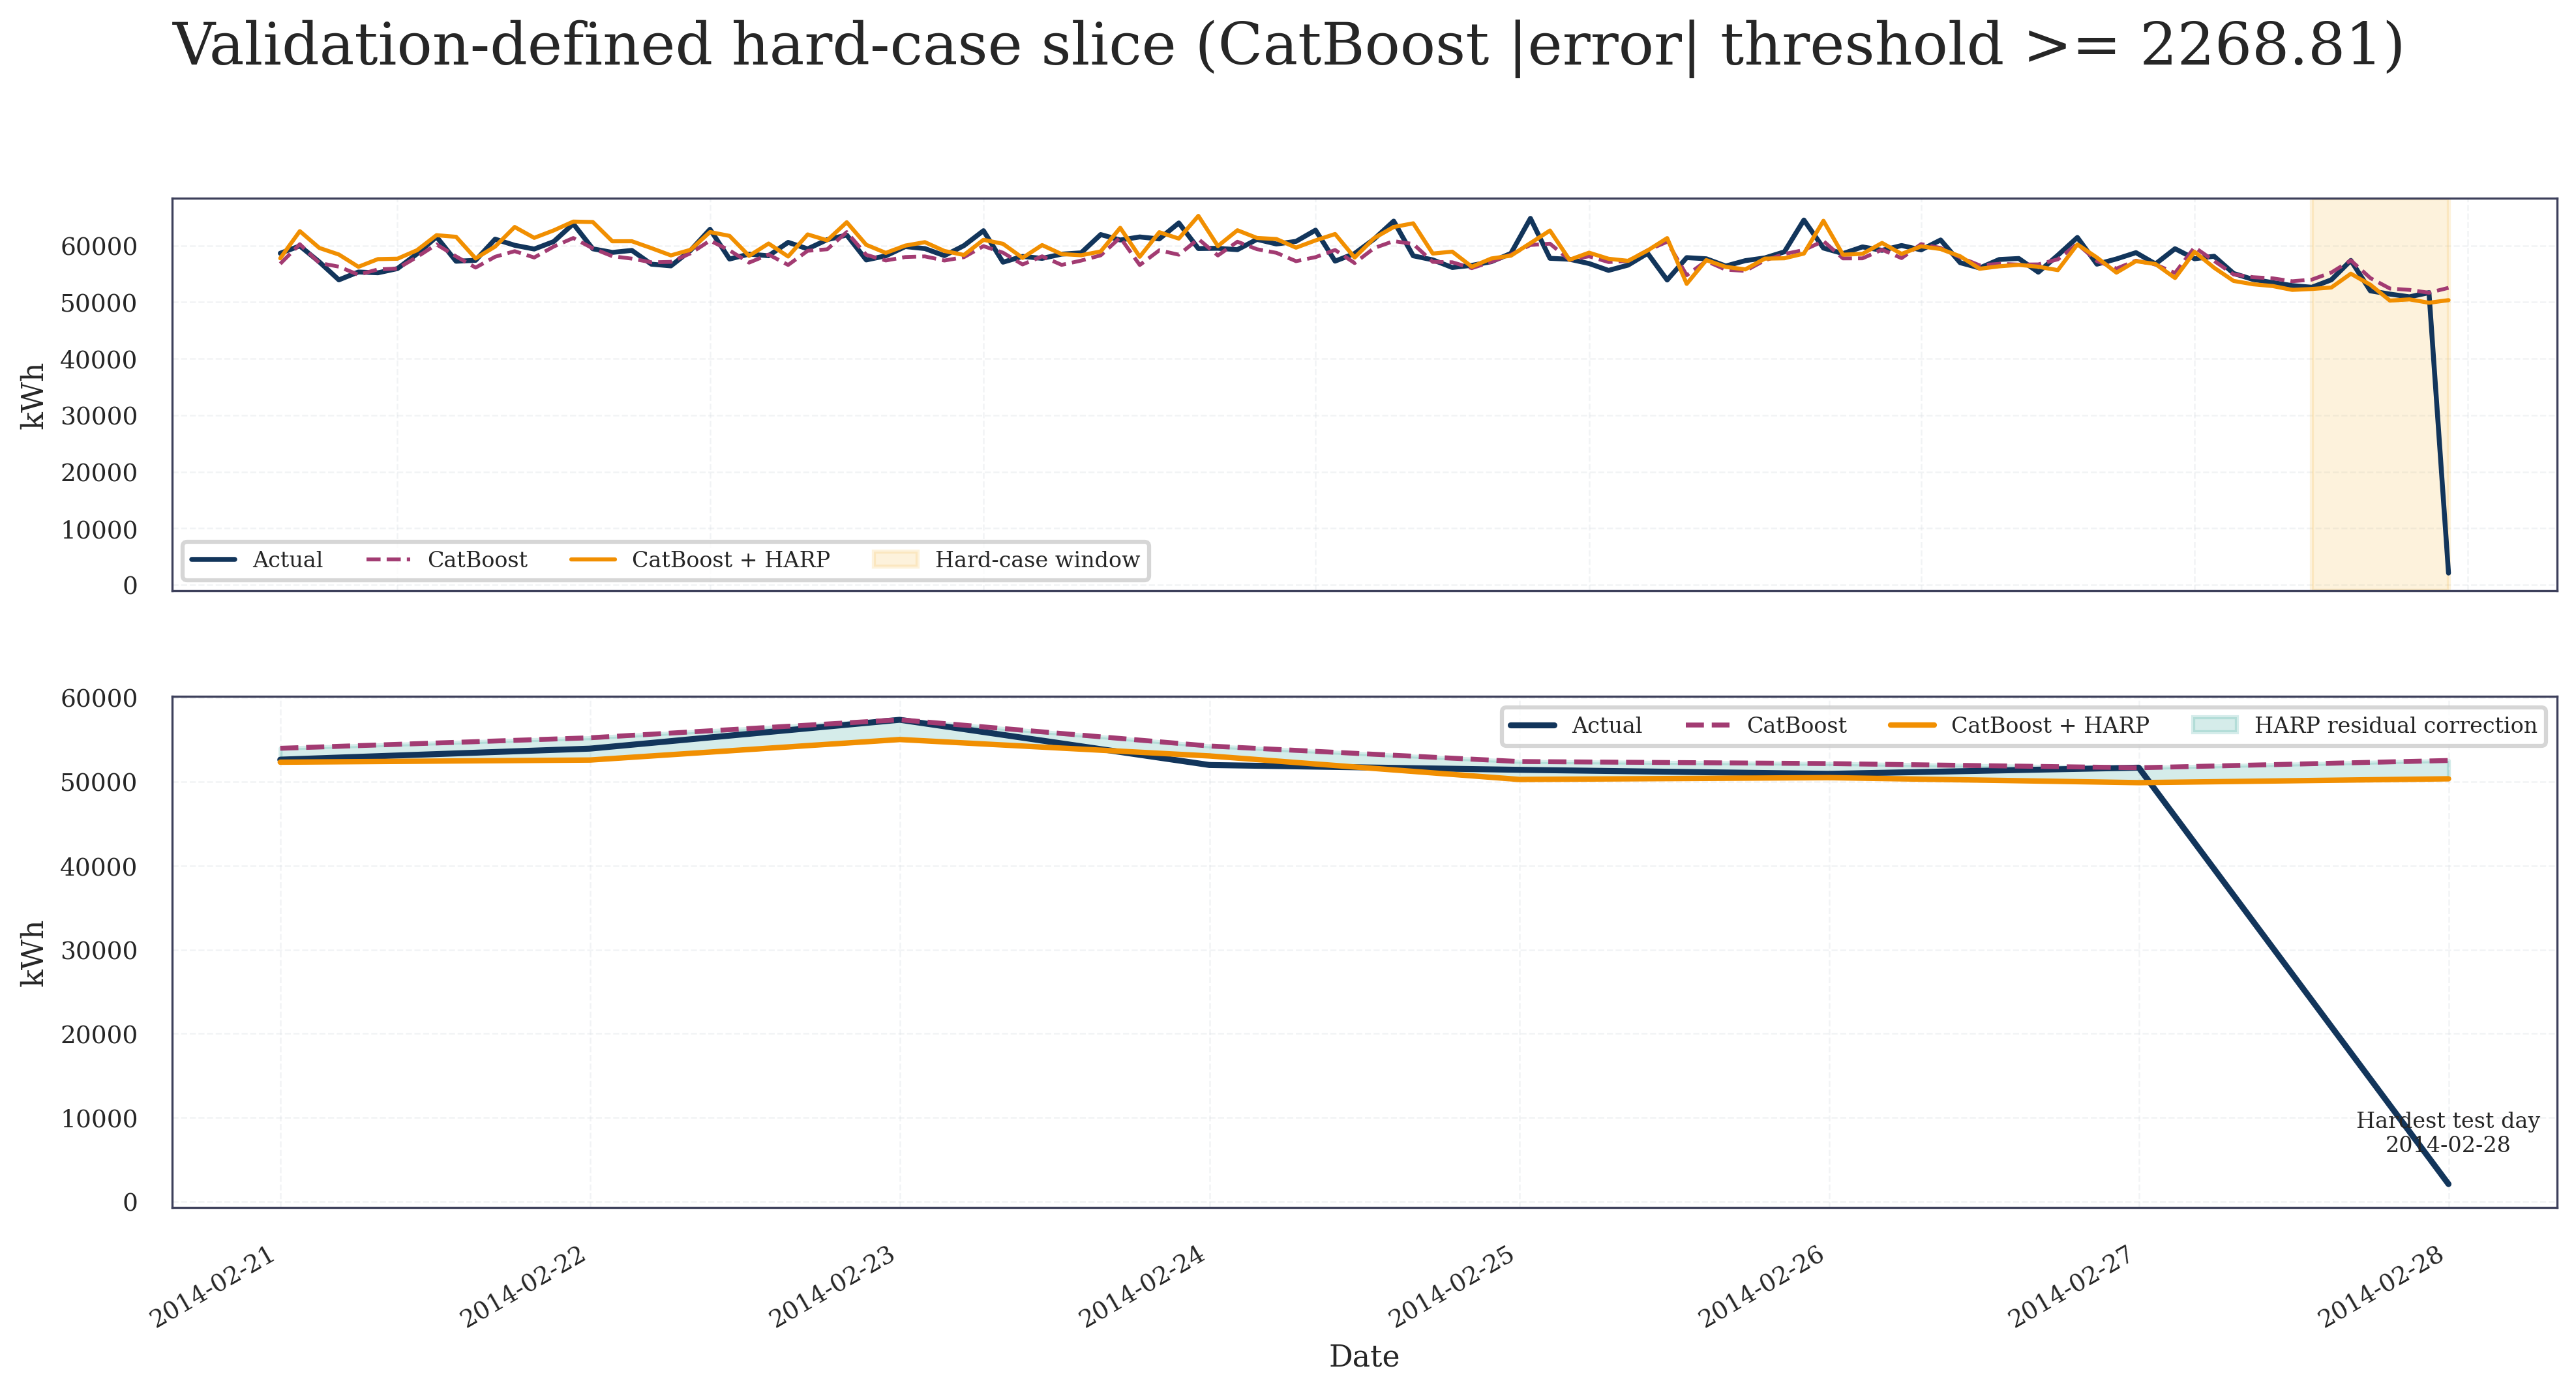
\includegraphics[width=0.94\textwidth]{hard_case_slice.png}
\caption{Validation-defined hard-case slice. The hardest errors are concentrated in a small number of days, and the hybrid model does not consistently repair them.}
\label{fig:hard_case_slice}
\end{figure*}

\begin{figure*}[t]
\centering
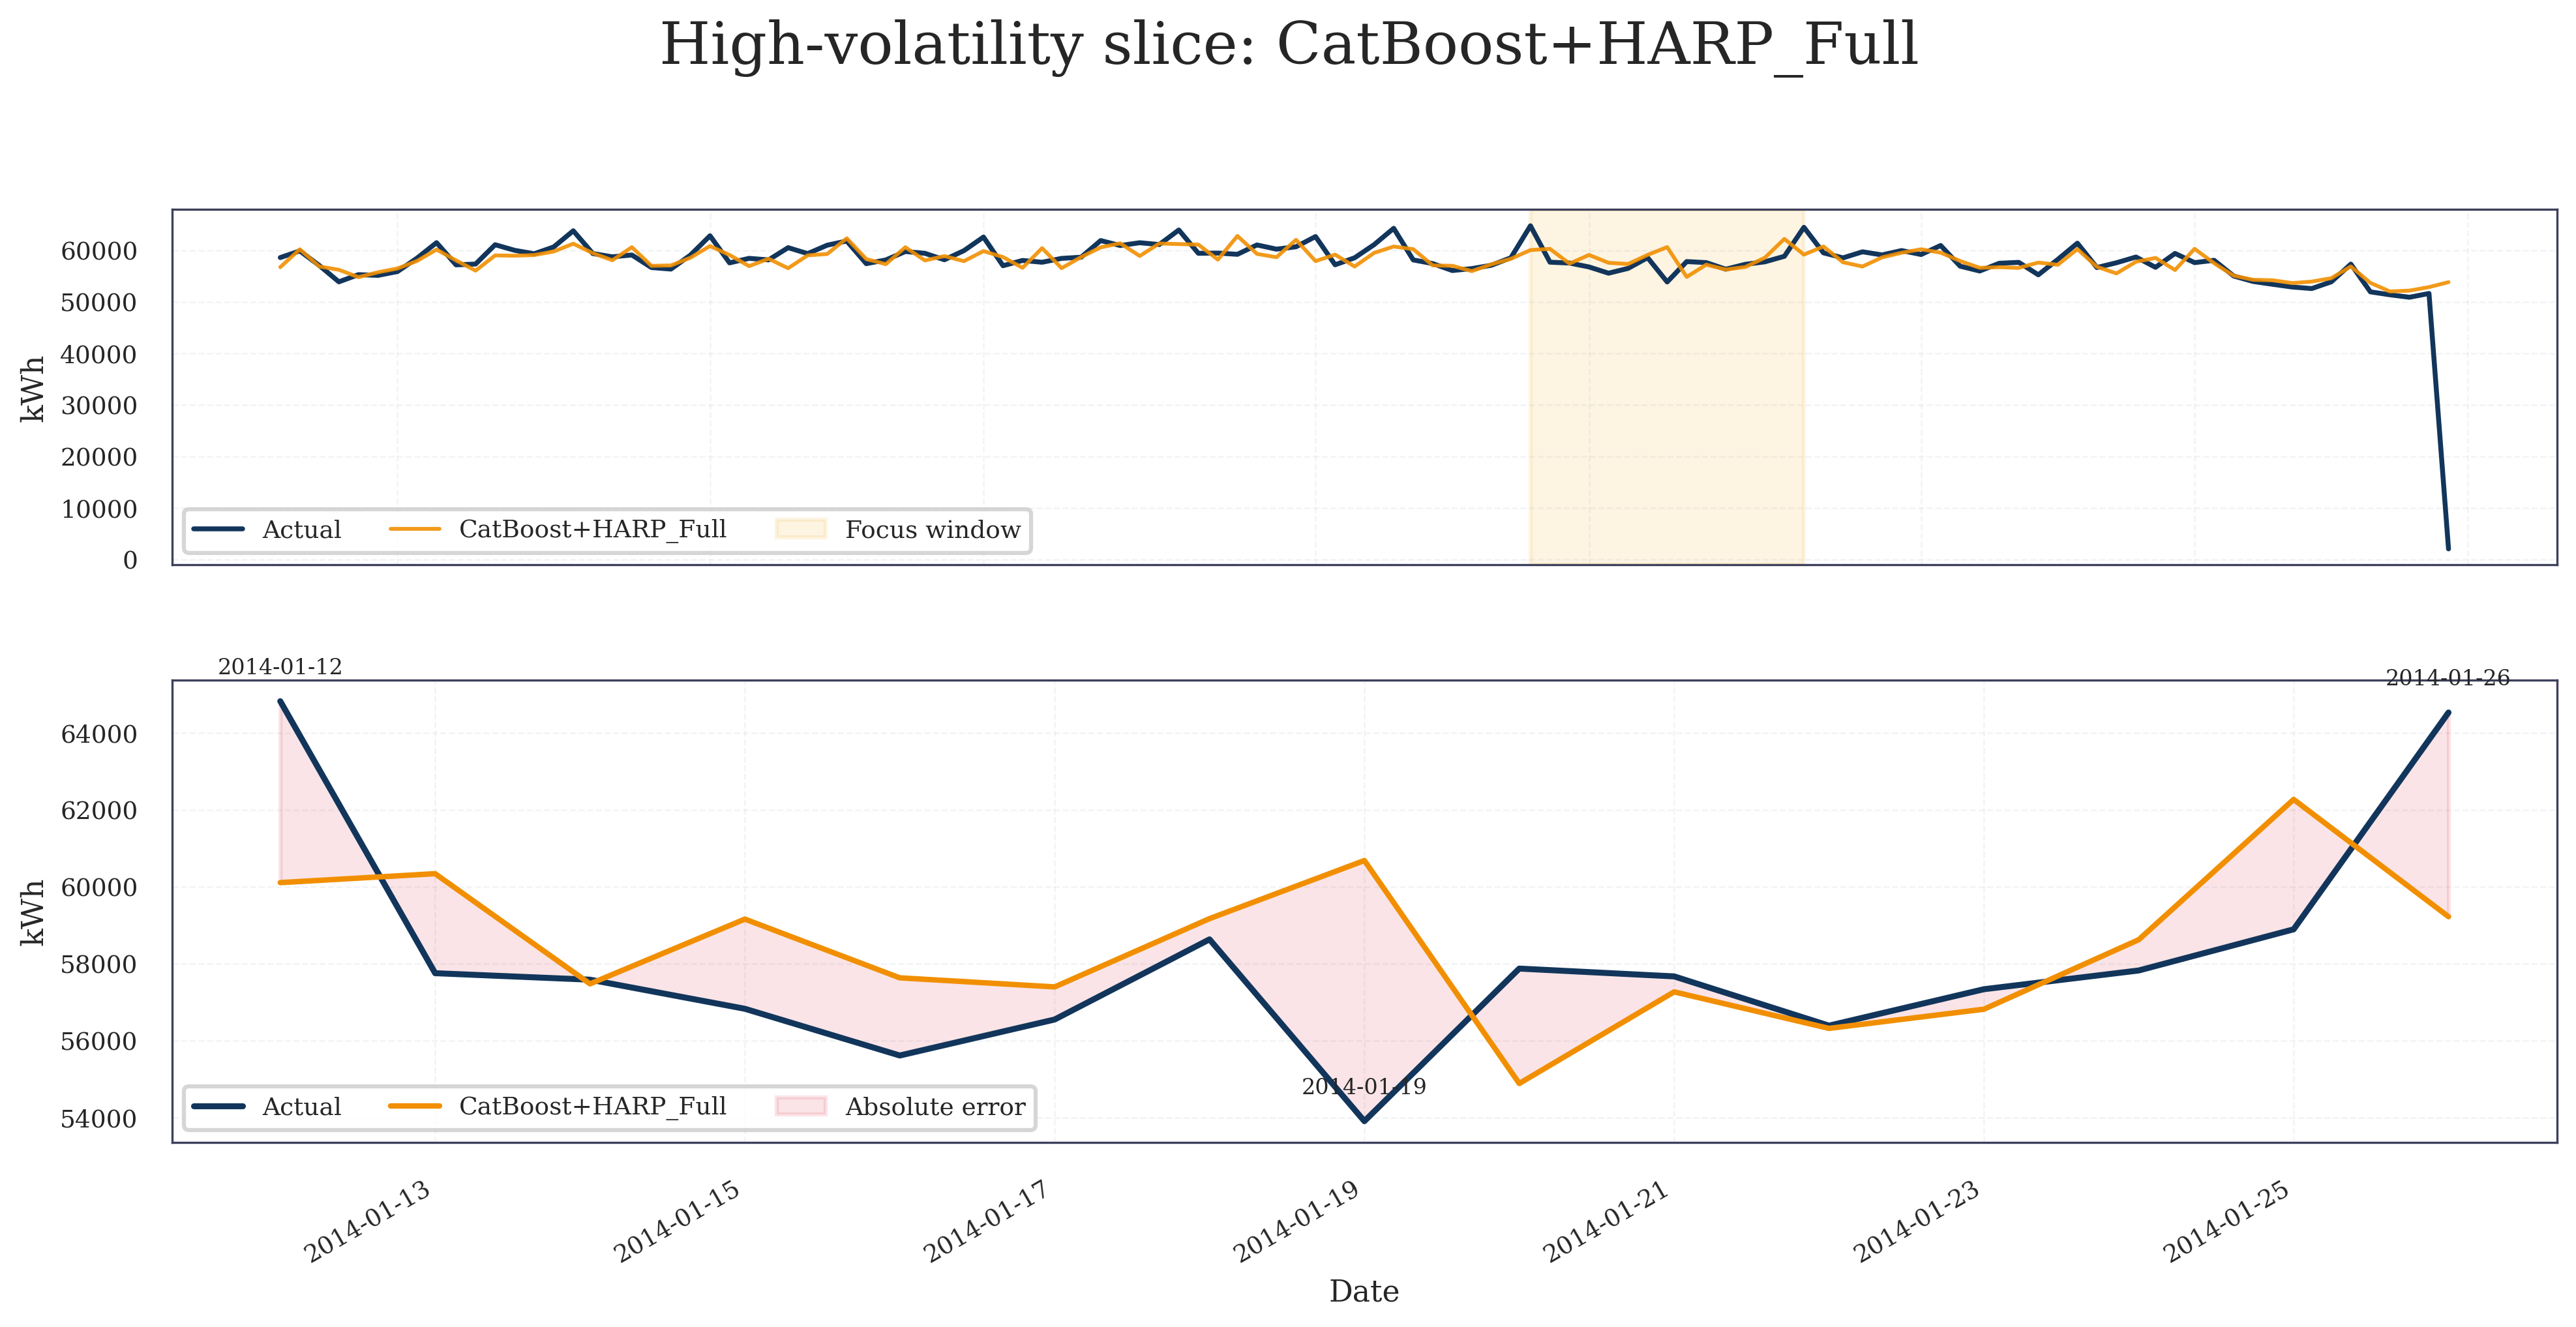
\includegraphics[width=0.94\textwidth]{high_volatility_slice.png}
\caption{High-volatility slice. CatBoost remains stronger in the most unstable periods of the series.}
\label{fig:high_volatility_slice}
\end{figure*}

The conclusion from the slice analysis is simple: the hybrid models do not lose because they are bad on every day. They lose because they are not strong enough on the difficult and unstable days that dominate RMSE.

\subsection{Interpretability and what it tells us}
One strength of the hybrid experiments is that they produce interpretable artifacts. CARE stores gate and confidence information, and the retrieval-based models show which past days were selected as analogs.

\begin{figure}[t]
\centering
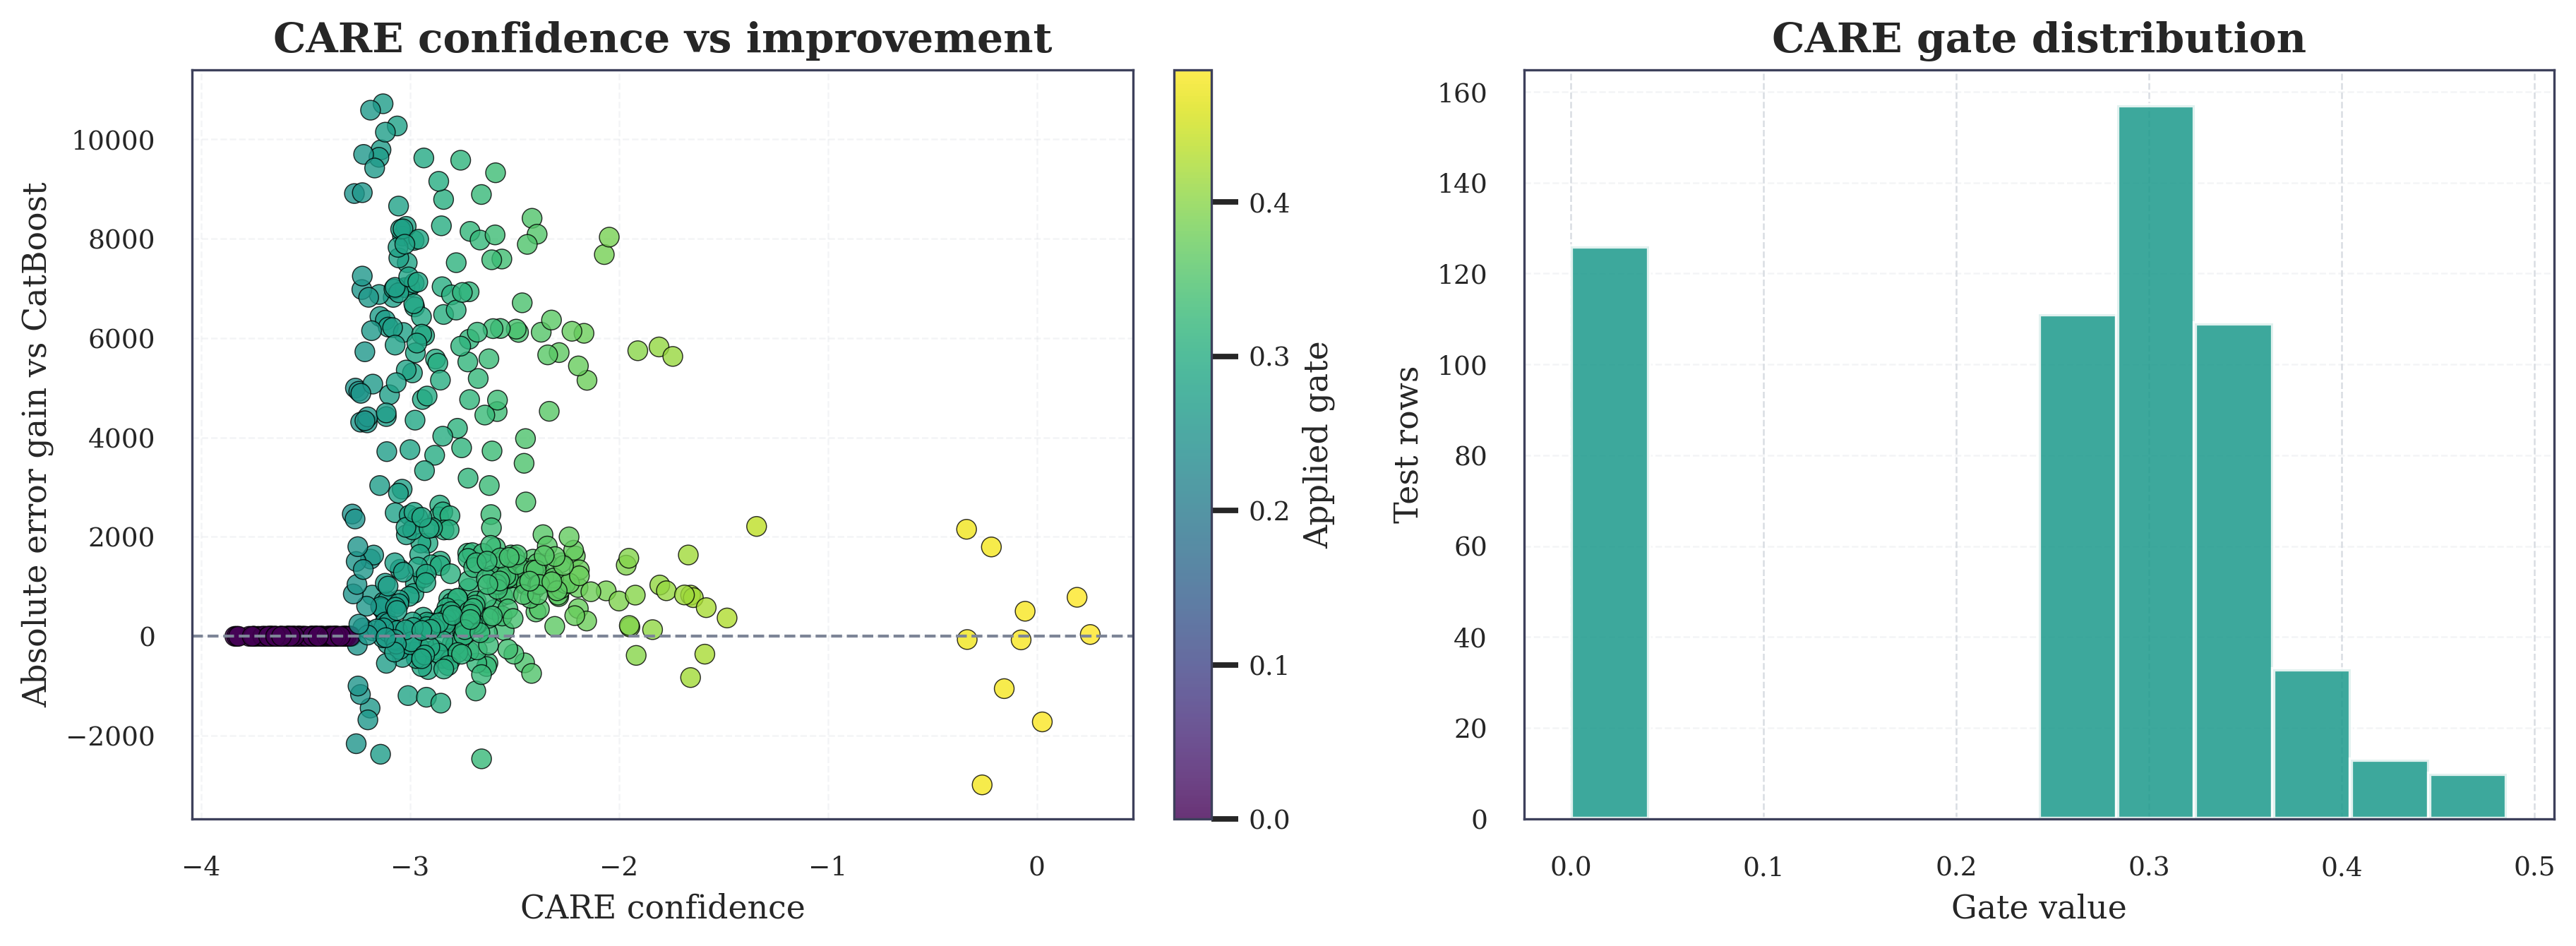
\includegraphics[width=\columnwidth]{care_confidence_vs_gain.png}
\caption{CARE confidence versus gain in absolute error. The gate behaves conservatively, but confidence is still not reliable enough to produce better overall RMSE than CatBoost.}
\label{fig:care_confidence_gain}
\end{figure}

\begin{figure}[t]
\centering
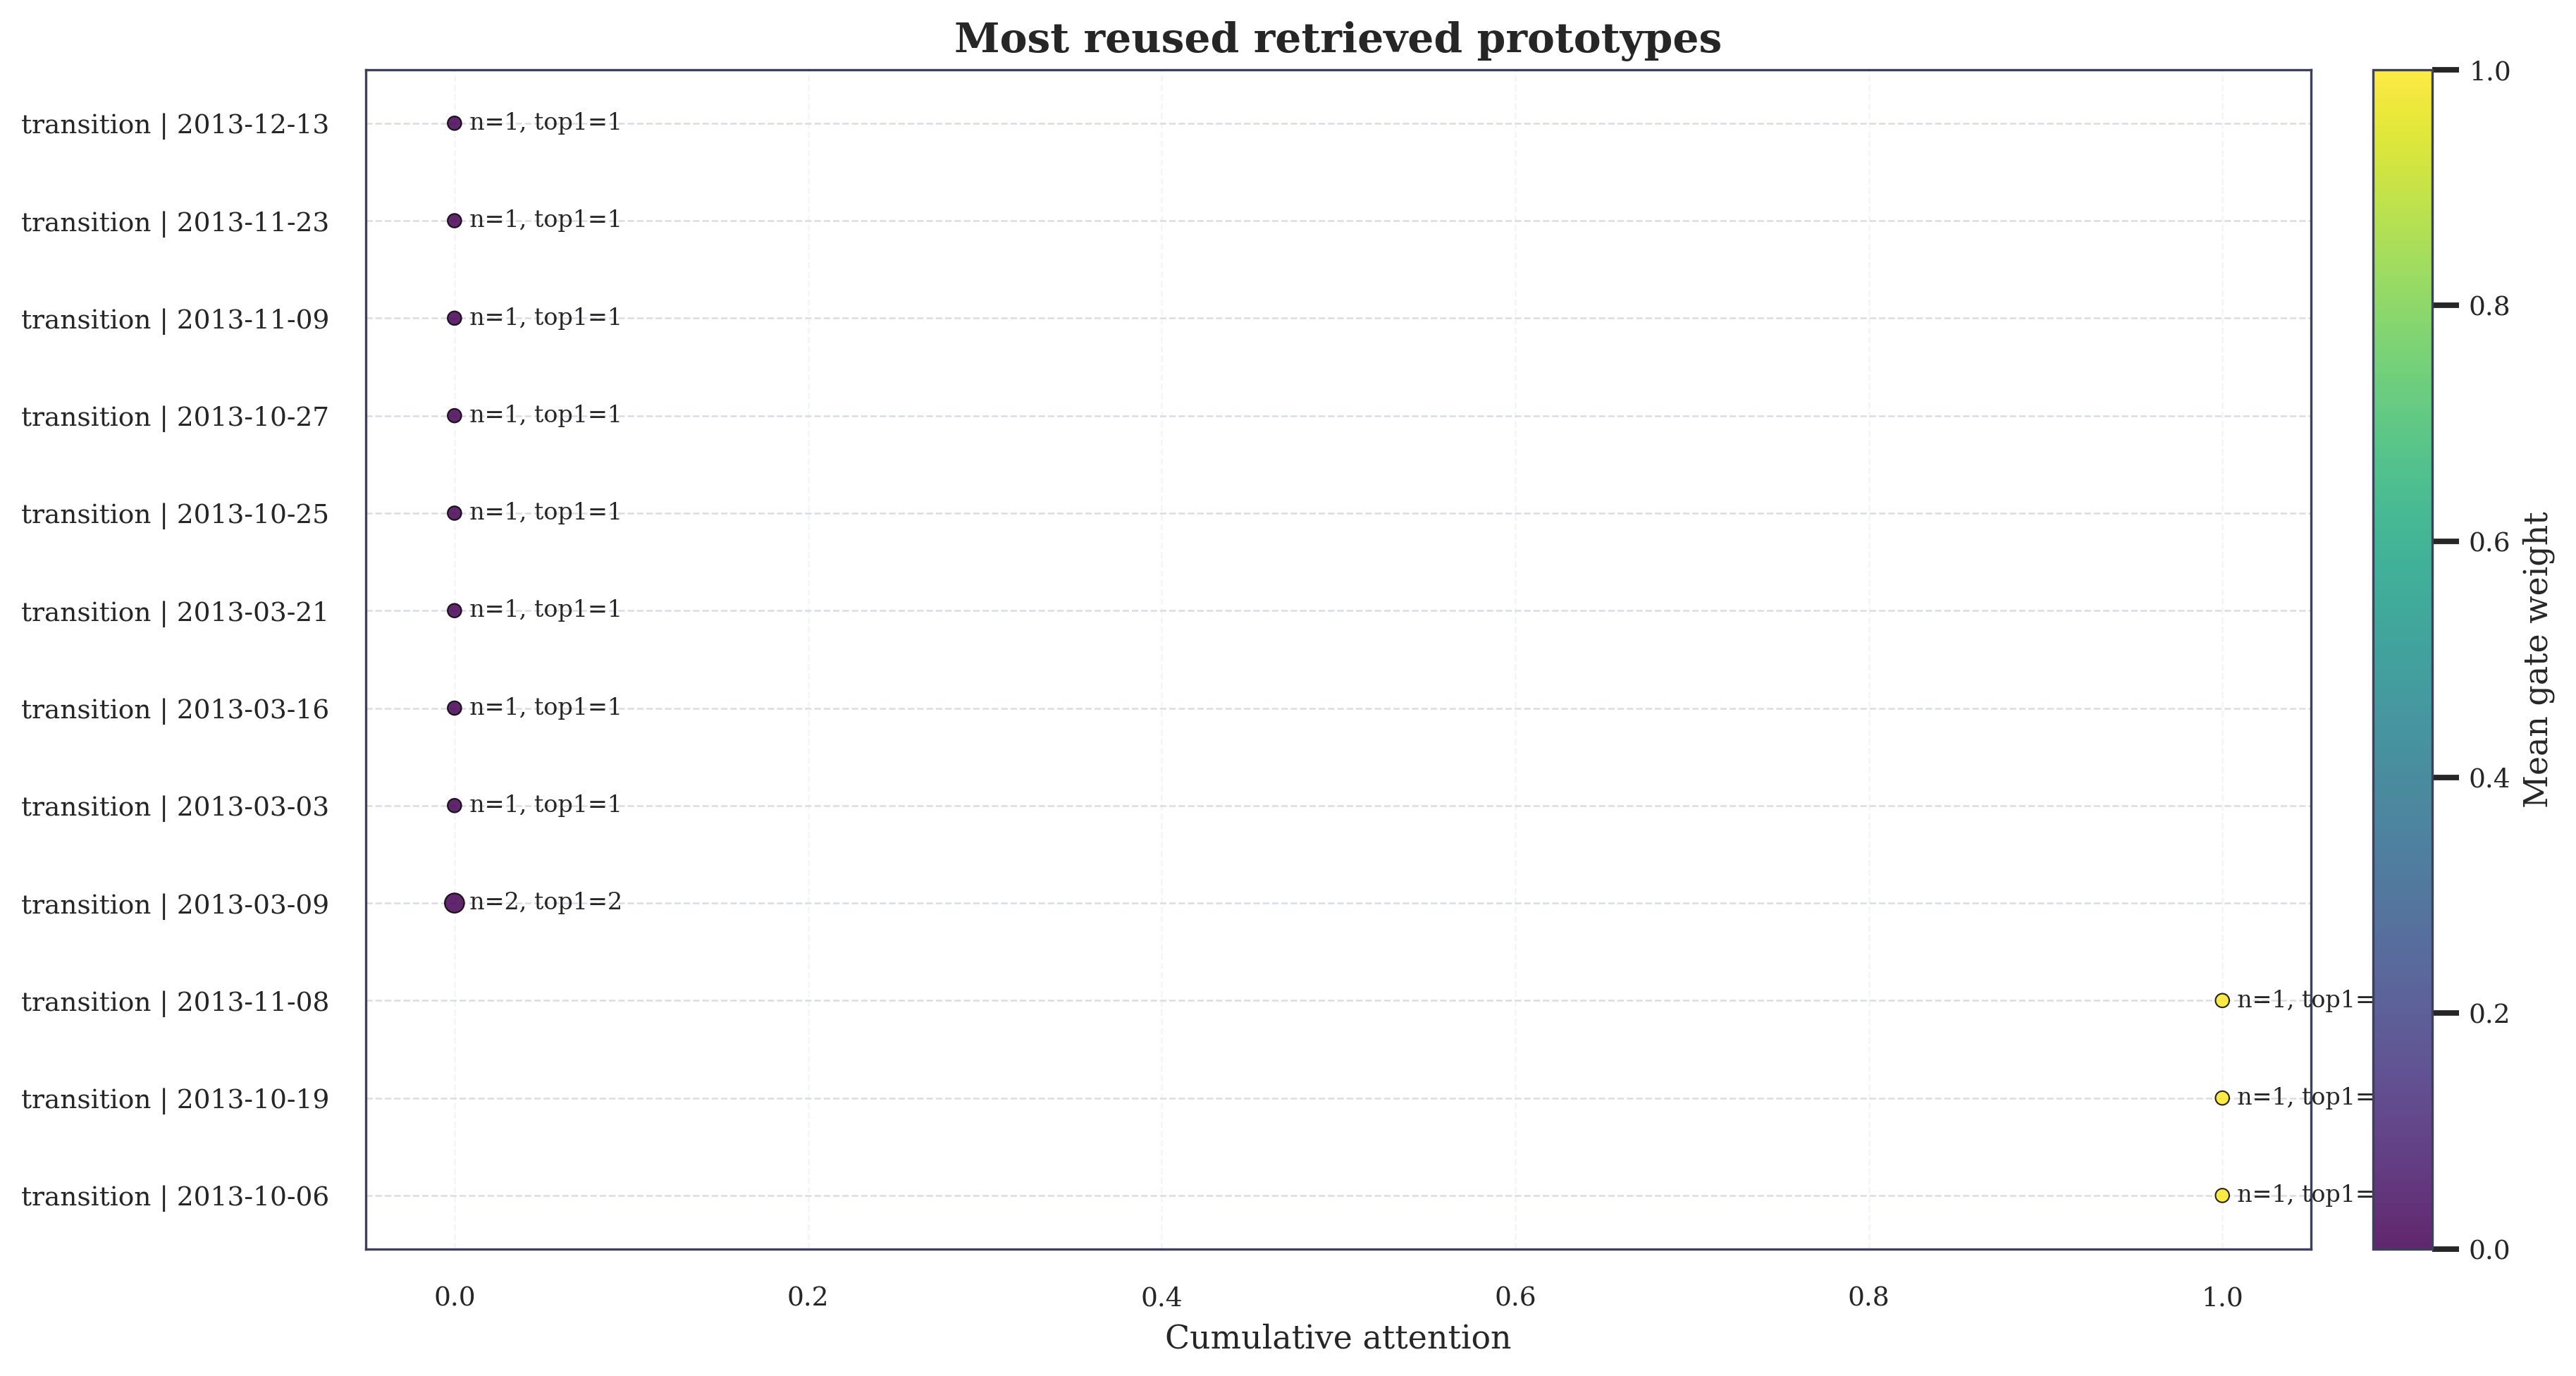
\includegraphics[width=\columnwidth]{retrieval_summary.png}
\caption{Retrieval summary from the hybrid pipeline. The retrieval mechanism is meaningful and interpretable, but retrieval quality alone is still not enough to beat the CatBoost backbone.}
\label{fig:retrieval_summary}
\end{figure}

These figures are useful because they show that the hybrid models are not random black boxes. They are making structured decisions. However, structured decisions are not the same thing as better final accuracy.

\section{Discussion}
\subsection{Why CatBoost is the best model for this dataset}
CatBoost wins because the project has already converted the time series into a strong supervised tabular learning problem. The model is given informative lag features, rolling statistics, and calendar indicators. In this setting, the main challenge is no longer ``discover hidden temporal structure from scratch.'' The challenge is ``learn stable nonlinear interactions from a small number of rows.'' That is exactly where CatBoost is strong.

CatBoost is also robust for this problem because it does not need a very large sample to become useful. It can learn from 517 training rows more effectively than a deep model that must learn internal sequence representations from limited data.

\subsection{Why the deep models did not win}
The deep models did not win for three practical reasons.

First, the dataset is too small for them to use their full representational advantage. Second, the strongest patterns are already visible in the engineered predictors. Third, the target is a single aggregate daily series, not a large multivariate high-frequency dataset.

This is an important conclusion for the study. The project did not fail to use deep learning correctly. Instead, the results show that deep learning was tested fairly and simply turned out not to be the best fit for this dataset.

\subsection{Why the hybrid models are still useful}
Even though the hybrid models did not beat CatBoost on RMSE, they are still useful in three ways.

First, they test a meaningful research question: can CatBoost's remaining error be corrected by a specialized residual model? Second, they provide interpretability through retrieval cases and gating logic. Third, they reveal the real problem more clearly than the main benchmark alone.

The hybrid experiments show that the remaining error is not mostly about average daily pattern learning. The real issue is a small set of difficult days where demand behaves very differently from the usual pattern.

\subsection{The shock-day problem}
The strongest single example is the final day in the test window, 28 February 2014. On that day, the actual load drops to 2084.53\,kWh while CatBoost predicts 52,532.52\,kWh. This is an extremely unusual event. Removing only this one point would reduce CatBoost RMSE from 5151.33\,kWh to 1961.47\,kWh.

This finding changes the interpretation of the whole project. The problem is not that the benchmark models are weak at normal-day prediction. The problem is that rare collapse-like or outage-like events dominate the squared-error metric. That is why the next useful research step is likely to be anomaly-aware forecasting or a special shock-day detection-and-fallback mechanism.

\subsection{Was the project approach correct?}
Yes. The approach used in this project is methodologically sound for the following reasons:
\begin{enumerate}
\item the dataset was validated before modeling,
\item the features were designed using only past information,
\item the split was strictly chronological,
\item strong baselines were included,
\item standard machine learning and deep learning models were compared fairly,
\item advanced hybrid models were tested only after identifying the best base model.
\end{enumerate}

This is exactly the right order for an academic forecasting project. It moves from simple to strong to advanced, without skipping the fairness checks.

\subsection{Simple summary for a non-specialist reader}
If a lay reader asks what happened in the project, the answer is:
\begin{enumerate}
\item a real smart-meter dataset was cleaned and converted into daily totals,
\item many forecasting models were tested fairly,
\item CatBoost worked best overall,
\item deep learning and hybrid models were explored carefully,
\item they did not beat CatBoost on the main metric,
\item the hardest remaining problem is rare shock-like days.
\end{enumerate}

\section{Threats to Validity}
This project has several limitations.

First, the study uses one aggregate daily series, not many separate series. That means the conclusion is strongest for this exact forecasting setup and should not be generalized blindly to every smart-meter problem.

Second, the training sample is small. This is the core reason for the project, but it also means that some model estimates may be sensitive to unusual periods.

Third, the project does not use external weather, tariff, holiday, outage, or occupancy variables. Some extreme days may only be explainable with such extra information.

Fourth, the hybrid models were explored within a fixed time and compute budget. More tuning might improve them. However, the current paper is honest about what was actually achieved, not what might happen after indefinite tuning.

At the same time, the study has real strengths. The leakage controls are explicit. The split logic is fair. The main metrics are validated from stored artifacts. The paper clearly distinguishes between inherited benchmark results and rerun hybrid results.

\section{Conclusion}
This paper presented a full and careful study of daily smart-meter forecasting on the Low Carbon London dataset. The project began with a simple question: which model is truly best for this dataset under a fair and leakage-safe setup? The answer is clear and well supported by the evidence: \textbf{CatBoost is the strongest overall model in the canonical setup}.

The study also tested whether residual hybrid refinements could improve over the CatBoost backbone. Dynamic retrieval came close. HARP-v2 improved MAE slightly but not RMSE. CARE improved some secondary behaviors, but it still did not surpass CatBoost on the main metric. These are not useless results. They show exactly where the remaining difficulty lies.

The main lesson of the project is simple. This dataset is better treated as a small tabular forecasting problem than as a large deep-sequence benchmark. The project approach was therefore correct: validate the data, prevent leakage, compare strong baselines fairly, and only then test more complex extensions. Future work should focus on rare shock-day handling, anomaly-aware correction, or external explanatory variables instead of simply increasing model complexity.

\bibliographystyle{IEEEtran}
\bibliography{bibliography}

\end{document}
